% % % % % % % % % % % % % % % % %
% `ctrl+F` goto 从这里开始
% % % % % % % % % % % % % % % % %
\documentclass[opening]{ecustbachelorthesis}

\begin{document}
% 文档初始化
\docinit
% 添加标题
\makethesistitle\makemyinfo
% 摘要
\begin{abstract}
\makeatletter\me@abstractzh\makeatother
\end{abstract}

% #从这里开始# 写开题报告
\section{研究背景}
\subsection{标题}
\subsubsection{标题}
一级标题(黑体小二号,居中,段前距为12磅),二级标题(宋体四号,段前距为12磅,段后距为0磅,接内容段前距为12磅),三级标题(黑体小四号,段前距为12磅,段后距为0磅),内容(首行缩进二格,宋体小四号)
\subsection{标题}
\subsubsection{标题}
表(宋体小五号粗体,按章编号,例如表2.7为第2章第7个表)
\begin{table}[!htbp]
  \centering
  \caption{林可霉素……}
  \label{tab:linc}
  \begin{tabular}{|c|c|c|c|}\hline
    第1行第1列 & 第1行第2列 & 第1行第3列 & 第1行第4列\\ \hline
    第2行第1列 & 第2行第2列 & 第2行第3列 & 第2行第4列\\ \hline
    第3行第1列 & 第3行第2列 & 第3行第3列 & 第3行第4列\\ \hline
  \end{tabular}
\end{table}

如表\ref{tab:linc}所示,这张表格为测试表格,标注格式规范文档。注意格式要求表名位于表格正上方,所以写论文时,要把\verb$\caption{...}$放在\verb$\begin{tabular}...$上面。

\section{文献综述}
\subsection{标题}
\subsubsection{标题}
数学公式(用斜体,按章编号),如公式\ref{eqn:abc}所示,这里可以用\verb$\ref{label}$来具体指代所说的公式,其中\verb$label$需要替换为上下文中设定label名字,例如在\verb$equation$中用\verb$\label{eqn:abc}$来设定该公式的标签(即\verb$label$)。
\begin{equation}
A=0.235B+2.68C \label{eqn:abc}
\end{equation}


\subsection{标题}
\subsubsection{标题}
图(图名位于图的正下方,用宋体小五号粗体,按章编号,图3-1为第3章第1个图)。如图\ref{fig:linc}所示,这张图为测试图,标注来自格式规范文档\cite{ecustjwc}。注意格式要求图名位于图片正下方,所以写论文时,要把\verb$\caption{...}$放在\verb$\includegraphics{...}$下面。
\begin{figure}[!htbp]
  \centering
  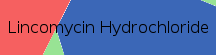
\includegraphics{img1}
  \caption{林可霉素……}
  \label{fig:linc}
\end{figure}

以上格式适用于论文、开题报告和文献翻译。参考文献使用bibtex工具,把文献按格式加入\verb$.bib$文件中,xelatex编译\verb$.tex$文件一次,用bibtex编译\verb$.aux$文件一次,再用xelatex编译\verb$.tex$文件2次。
\section{技术路线}
\section{进度安排}

% 最后的参考文献
\bibliography{opening}
\end{document}
